\documentclass[a4paper]{article}

%% Language and font encodings
\usepackage[english]{babel}
\usepackage[utf8x]{inputenc}

\usepackage[T1]{fontenc}
\usepackage{wrapfig, blindtext}

%% Sets page size and margins
\usepackage[a4paper,top=3cm,bottom=2cm,left=3cm,right=3cm,marginparwidth=1.75cm]{geometry}

%% Useful packages
\usepackage{amsmath}
\usepackage{graphicx}
\usepackage[colorinlistoftodos]{todonotes}
%Color a las referencias
\usepackage[colorlinks=true, allcolors=blue]{hyperref}
%Color a los textos

%Caratula
\begin{document}
\begin{titlepage}
\begin{center}
\vspace*{-0.4in}

{\fontsize{12}{30}\bf \selectfont UNIVERSIDAD NACIONAL DE INGENIERIA\\}

{\fontsize{12}{40}\bf \selectfont FACULTAD DE CIENCIAS\\}
\vspace*{0.15in} CIENCIAS DE LA COMPUTACI\'ON\\
\vspace*{0.2in}


\begin{center}

\includegraphics[width=5.5cm,height=6.5cm]{UNI.png}
\end{center}
\vspace*{0.2in}

\begin{large}
	{\bf PROYECTO DE BIOLOGIA COMPUTACIONAL\\}
	\vspace*{0.3in}
\end{large}

\begin{large}
{\bf T\'itulo del Trabajo\\}
\vspace*{0.2in}
\end{large}

\begin{Large}
\color{blue}
\textbf{Creación de un sistema de ayuda para el analisis de información Genética de Especies endémicas de las regiones del Perú\\}
\color{black}
\end{Large}
\vspace*{0.2in}

\begin{large}
{\bf Autores} 
\vspace*{0.1in}
\\L\'azaro Camasca, Edson Nicks\\
Leon Rios, Marco Naro
\end{large}
\vspace*{0.4in}


\begin{large}
{\bf Profesor} 
\vspace*{0.1in}
\\Nuñez Iturri, Ciro Javier
\end{large}

\end{center}
\begin{center}
\begin{large}
\vspace*{1.0in}
Lima - Peru\\
{\bf (2019)}
\end{large}
\end{center}
\end{titlepage}

\pagebreak
\tableofcontents
\pagebreak

\section{Objetivos}

\subsection{Objetivos Generales}
\begin{itemize}
\item  Creación de un software grafico con una base de datos para el analisis de infomacion genética.
\end{itemize}

\subsection{Objetivos Especificos}
\begin{itemize}
\item Recolectar informacion genetica de especies endemicas.

\item Desarollar la aplicación  para el analisis de secuencias,.

\item Desarrollar algoritmos para obtener árboles filogenéticos 

\item Evaluar el árbol filogenético
\end{itemize}

\section{Resumen Ejecutivo}

Se pretender crear un software y una base de datos con la informacion genetica de las especies endemicas del peru, el software procesara las secuencias, crara el árbol filogenético, mostrara los resultados y analizara las relaciones evolutivas de las especies escogidas.

\section{Descripción del Proyecto}

El proyecto sera implementado netamente en el lenguaje Pyhton
Las librerias utilizadas seran:
\begin{itemize}
\item BioPython para el procesamiento de secuencias
\item Tkinter o Gt para el entorno grafico.
\end{itemize}
Dentro de la GUI, se pobra escoger /Especie/Genes/Proteina para el análisis posterior.\\
Los datos recolectados seran reales de la base de datos de NCBI.\\
Se implementara algoritmos para el alineamiento de Genes homólogos.\\
Se implementara algoritmos para el alineamiento de Proteinas.\\
Se implementara la algoritmos para la Generacion de Arboles Filogenticos de acuerdo a un modelo.\\

\noindent Para el desarrollo del proyecto se seguira la siguiente metodologia:

\subsection{Determinar las secuencias a utilizar}
El alineamiento de secuencias debe permiter la determinación de regiones homologas 
\subsection{Elegir los marcadores moleculares}
\subsection{Realizar el lineamiento multiple de genes homologos}
\subsection{Elegir un modelo evolutivo}
Entre los modelos tenemos:

\begin{itemize}
\item Modelo Jukes-Cantor: asumiento que los nucleotidos son substituidos con igual probabilidad
\item Modelo Kimura: realista ya que considera las diferentes tasas de mutación
\end{itemize}
\subsection{Aplicar un método para la construcción del árbol filogenético}	
Entre los metodos tenemos 
\begin{itemize}
	\item Basados en distancia
	\item Basados en secuencia
	\item Basados en agrupamiento
	\item Basados en optimalidad
	\item Basados en caracteres
\end{itemize}

\subsection{Verificar la fiabilidad del árbol construido}

\subsection{Analizar el arbol filogenetico}
Apartir del arbol filogenetico se podra descubrir/Mostrar/Analizar las relaciones evoluticas de las especies endemicas escogidas.
\subsubsection{Modelamiento de la Estrutura de Proteinas}
En el analisis se encuentra el modelamiento de la Estructura de Proteinas

\subsection{Cronograma}
Para el desarollo del proyecto se emplea un cronograma por semanas, las fechas del cronograma coinciden con las fechas propuestas para evaluaciones de práctica del proyecto. En dichas ocaciones se presentarán y evaluarán los avances del proyecto.

\begin{center}
	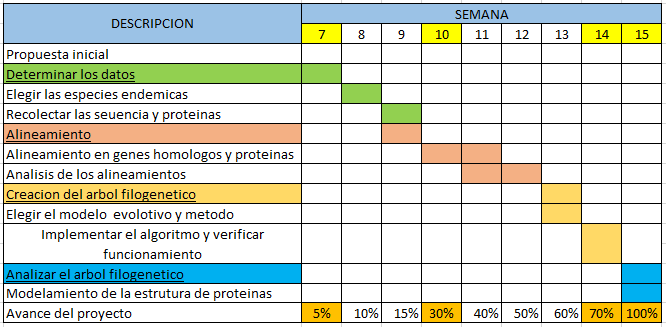
\includegraphics[width=14cm,height=8cm]{cronoextendido.png}\\
	Fig: Cronograma por semanas	
\end{center}

\begin{center}
	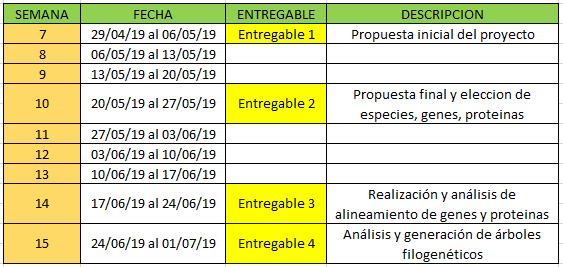
\includegraphics[width=10cm,height=6cm]{cronoentregrable.png}\\
	Fig: Cronograma coincidente a los entregables
\end{center}


\vspace*{0.2in}


\section{Algoritmos e implementación computacional}
Una descripcion de los algoritmos y herramientas que se [planean utilizar en caso de la propuesta] utilizados incluyendo pseudo código y codigo fuente
\section{Resultados}
Una descripción de los resultados [esperados en el caso de la propuesta]. Un reporte integrando los resultados proporcionados por la herramienta
\section{Conclusiones}
Incluye las ventajas y desventajas del enfoque utilizado, aspectos inesperados del proyecto, trabajo futuro, etc.
\section{Apéndice}


\end{document}